\documentclass[sigconf,nonacm]{acmart}

% ---- Packages ----
\usepackage{booktabs,graphicx}
\usepackage{amsmath}
\usepackage{makecell}
\usepackage{tikz}
\usetikzlibrary{positioning,arrows.meta}
\usepackage[capitalize]{cleveref}
\usepackage{microtype}                 % char protrusion + font expansion: fixes text spilling past the margin
\setlength{\emergencystretch}{3em}     % allow extra glue on hard lines so nothing overflows the text block

% ---- acmart housekeeping (nonacm) ----
\settopmatter{printacmref=false}
\setcopyright{none}
\pagestyle{plain}
\graphicspath{{figures/}}

\begin{document}

% ---- Title / authors ----
\title{The Benchmark Chooses the Winner: Operating Points, Fine-Tuning, and the Fragility of Safety-Guard Rankings}
\subtitle{A Fair, Reproducible Evaluation of Small LLM Guards}

\author{Anonymous}
\affiliation{%
  \institution{Anonymous}
  \country{}
}

\begin{abstract}
Safety guards are typically compared by a single F1 computed at each model's own decision threshold. We show this turns the ranking into an artifact of the operating point: the reported winner changes with the threshold, the metric, and the benchmark. Treating that as the central measurement problem, we study a small, laptop-trained guard --- SmolLM3-3B fine-tuned with LoRA into a one-forward-pass \{safe, unsafe\} classifier --- under an operating-point-fair protocol: threshold-free AUPRC/AUROC, a matched-FPR operating point, and paired-bootstrap 95\% confidence intervals (CIs) with McNemar tests. Building this protocol also surfaced and fixed real evaluation bugs in our own first pipeline (calibration leakage, batch-amortized latency, an asymmetric per-model threshold advantage, and a baseline error-handling bias).

Three results make the thesis concrete. First, native-threshold F1 is rank-inverting: two open guards swap order between their native F1 and threshold-free AUPRC. Second, a base-vs-tuned decomposition shows parameter-efficient fine-tuning specializes in-distribution while \emph{degrading} out-of-distribution ranking --- on four novel benchmarks the \emph{untuned} base outranks the tuned guard (aggregate AUPRC 0.886 vs 0.781, non-overlapping CIs) at equal peak F1, so the guard's out-of-distribution lead is inherited base competence rather than a product of tuning. Third, an \emph{exploratory}, seed-scale mortgage case study illustrates that the winner is benchmark-dependent: a saturated in-domain benchmark ranks every system near the ceiling, whereas a hardened, trap-typed rebuild de-saturates the field --- small guards over-block benign-but-risky prompts far more than a frontier model, and the in-domain fine-tune that leads \emph{here} is the reverse of the general-OOD result where the untuned base leads. Under the fair protocol the guard still beats Llama-Guard-3-1B decisively (non-overlapping CIs, including out-of-distribution) and ties gpt-5.4-mini on F1 at lower batch=1 latency: an efficiency result, not an accuracy one.
\end{abstract}

\maketitle

\section{Introduction}

Large language models are now deployed as chat assistants and autonomous agents, where a single unsafe completion, a successful jailbreak, or an over-eager refusal all carry real cost. The dominant mitigation is a \emph{safety guard}: a classifier that screens content --- most commonly user prompts, and in some systems model responses --- as \texttt{safe} or \texttt{unsafe} before it reaches the model or the outside world. We are explicit up front about scope: our guard and \emph{every} evaluation in this paper classify \textbf{input prompts}. Screening of model \emph{responses} and of \emph{agent} tool-call arguments or tool outputs --- the surfaces that motivate the ``agent-bouncer'' name --- is \emph{not} evaluated here and is left to future work (\S\ref{sec:future}). In practice, teams face an unattractive choice. Purpose-built open guards (Llama Guard 1/2/3 and Prompt Guard, ShieldGemma, Aegis, Granite Guardian, WildGuard) are convenient but are often reported on their own favorable operating points; proprietary frontier classifiers are strong but add per-request cost, latency, and a data-sharing dependency. Meanwhile, published guard comparisons frequently tune a threshold for the proposed system while holding baselines at fixed points, report latency as batch-amortized throughput, and decontaminate with exact string matching --- choices that quietly inflate the reported advantage.

This paper is a \textbf{measurement and controlled-study} contribution, not a state-of-the-art chase. We fine-tune SmolLM3-3B into a binary guard that emits a single-token verdict --- a softmax over the \texttt{\{safe, unsafe\}} token logits at the last position, i.e.\ one forward pass --- with temperature and decision threshold calibrated on an \emph{in-distribution} dev split only (in-house held-out and novel benchmarks contribute zero rows to calibration). Training is parameter-efficient LoRA (r=32, all seven projections; 60.5M trainable params, 1.93\% of 3.14B) run in \textasciitilde{}71 minutes / 300 steps on a single consumer Apple M4 Max laptop (36 GB unified memory, MPS backend, no CUDA). Everything --- training, calibration, and evaluation --- fits on a laptop, so the protocol is cheap to reproduce and audit.

Our emphasis is on \emph{how} we measure, and we are careful with the word ``held-out,'' which we split into two distinct pools throughout the paper:

\begin{itemize}
  \item \textbf{In-house held-out} --- two of our six in-house benchmarks (JailbreakBench, XSTest) are held out from training and calibration but drawn from the same overall pool.
  \item \textbf{Novel held-out (OOD)} --- four benchmarks from source families the guard never saw during training (WildGuardTest, WildJailbreak, OR-Bench-Hard, HarmBench).
\end{itemize}

We evaluate on 6 in-house benchmarks (2,018 balanced, leakage-filtered test rows across guardrail, red-team, and over-refusal axes) and on the 4 novel held-out benchmarks (2,020 balanced rows across three sets, plus 200 all-harmful HarmBench rows). We compare against gpt-5.4-mini, Llama-Guard-3-1B, ShieldGemma-2b, and a keyword matcher, using paired-bootstrap 95\% CIs, McNemar tests, threshold-free AUPRC/AUROC, and a matched-FPR@0.10 operating point, with latency measured at true batch=1. Building this pipeline surfaced real bugs in our own first evaluation --- a calibration leak, batch-amortized latency, an asymmetric threshold advantage for our own model, and an API-error default that biased the GPT baseline's FPR --- which we document and fix.

The headline comparisons are collected once in \Cref{tab:headline} and reported in full, with CIs, in \S\ref{sec:results}; we do not restate them in prose. The one-line reading: under the fair protocol the guard leads the open guards on threshold-free AUPRC --- decisively over Llama-Guard-3-1B (non-overlapping CIs), including on the four novel benchmarks --- and ties gpt-5.4-mini on F1 at lower batch=1 latency. But the load-bearing finding is not the guard's standing; it is that the standing is contingent on the operating point, and that the tuning credited for it does not survive out of distribution: the \emph{untuned} base outranks the tuned guard on the novel benchmarks (\S\ref{sec:base-vs-tuned}).

\begin{table*}[t]
  \centering
  \small
  \caption{Headline results (in-house pooled unless noted). Only the guard's pooled/held-out AUPRC, the guard-vs-Llama novel aggregate, the base-vs-tuned delta, and the GPT $\Delta$F1 carry CIs; baseline AUPRCs are point estimates.}
  \label{tab:headline}
  \begin{tabular}{lllll}
    \toprule
    Metric (in-house pooled unless noted) & Guard & Llama-Guard-3-1B & ShieldGemma-2b & gpt-5.4-mini \\
    \midrule
    AUPRC & 0.844 [0.825, 0.866] & 0.639 & 0.712 & --- \\
    AUPRC, 4 novel held-out (aggregate) & 0.781 [0.751, 0.811] & 0.701 [0.673, 0.733] & pending & --- \\
    Matched-FPR@0.10 F1 & 0.581 & 0.360 & 0.464 & --- \\
    F1 (paired vs guard) & tie ($\Delta$F1 +0.010, $p=0.20$) & --- & --- & native point 0.784 \\
    Latency, batch=1 p50 & 124 ms & not measured & not measured & \textasciitilde{}512 ms (remote API) \\
    \bottomrule
  \end{tabular}
\end{table*}

Only the guard's pooled/held-out AUPRC, the guard-vs-Llama novel aggregate, the base-vs-tuned delta, and the GPT $\Delta$F1 carry CIs; baseline AUPRCs are point estimates (see \S5, \S6).

We are explicit about limits. Matched-FPR@0.10 makes every system conservative (guard recall 0.431 there), so AUPRC is our fair primary summary; at the \emph{deployed} operating point (T=2.10, $\tau=0.59$) the guard's overall FPR is 0.306, i.e.\ it over-blocks benign prompts, which we treat as a real deployment concern. ShieldGemma is run somewhat outside its designed content-policy regime and its novel-benchmark numbers are still pending; a single global threshold is structurally in-distribution-optimized. Positioned against the two closest works, we complement CPU-class efficient-guard studies (``Do You Really Need a GPU to Guard Your LLM?'') by adding rigorous operating-point-fair comparison and a base-vs-tuned decomposition on a 3B generative guard, and we serve as the constructive counterpart to ``Why LLM Safety Guardrails Collapse After Fine-tuning'' (ICML 2025): where they show tuning can destroy alignment, we show that even when tuning \emph{works}, its measurable gains are memorized in-distribution and do not transfer to the in-house held-out sets we can test.

\subsection{Contributions}

\begin{itemize}
  \item \textbf{Operating-point-fair evaluation.} We show guard rankings depend heavily on the decision threshold, so naive per-model-threshold comparisons are misleading; we instead report matched-FPR@0.10, threshold-free AUPRC/AUROC, and paired-bootstrap CIs with McNemar tests.
  \item \textbf{A base-vs-tuned decomposition.} An instruction-tuned 3B base already carries most of the safety-classification competence measurable on our in-house benchmarks by F1 (its zero-shot F1 beats both open guards'); parameter-efficient tuning specializes in-distribution and does \emph{not} meaningfully improve the two in-house held-out benchmarks we can measure (macro $-0.005$), and slightly regresses over-refusal.
  \item \textbf{A domain stress test of the same effect (exploratory).} On a mortgage fair-lending task we show a benchmark can be \emph{saturated} --- a zero-shot 3B base is already near-ceiling, so every system looks excellent and none can be ranked --- and we rebuild it as a hardened, trap-typed set that de-saturates the field: small guards over-block benign-adjacent prompts far more than a frontier model, and which fine-tune ``wins'' flips between this in-domain set and the general novel sets. We flag this as a seed-scale, single-annotator case study rather than a headline result (\Cref{sec:mortgage-casestudy}).
  \item \textbf{A small, local, laptop-trained guard.} On threshold-free AUPRC it surpasses purpose-built open guards --- Llama-Guard-3-1B decisively (non-overlapping CIs), \emph{including} on the novel held-out benchmarks, and ShieldGemma-2b on the in-house pooled / in-dist / in-house-held-out sets (ShieldGemma's novel runs are pending) --- and it matches frontier gpt-5.4-mini on F1 at \textasciitilde{}4$\times$ lower latency.
  \item \textbf{A rigorous, reproducible, laptop-scale protocol.} Paired CIs, McNemar, matched-FPR, and family-level decontamination --- a pipeline that exposed real evaluation bugs in our own first attempt --- released as open code (the evaluation scripts plus a single orchestrating reproduction notebook).
\end{itemize}

\section{Related Work}

\textbf{LLM safety guards and content moderation.} A growing family of purpose-built classifiers screens prompts and responses for LLM and agent pipelines. Meta's Llama Guard line (1/2/3) \cite{inan2023llamaguard,meta2024llamaguard2_3,fedorov2024llamaguard3_1b} and Prompt Guard \cite{meta2024promptguard}, Google's ShieldGemma \cite{zeng2024shieldgemma}, NVIDIA's Aegis \cite{ghosh2024aegis}, IBM's Granite Guardian \cite{padhi2024graniteguardian}, and AI2's WildGuard \cite{han2024wildguard} all frame moderation as a supervised classification task over a safety taxonomy, typically emitting a verdict token or category label. Recent work pushes on the \emph{reasoning} axis (R\textsuperscript{2}-Guard's knowledge-enhanced logical-reasoning inference \cite{kang2025r2guard} at ICLR 2025, DuoGuard's two-player RL/multilingual training \cite{deng2025duoguard}, and other reasoning-guards). Our guard is deliberately minimal by comparison: a single-token verdict read from the \{safe, unsafe\} logits in one forward pass, LoRA-tuned (60.5M trainable params, 1.93\% of 3.14B) on a consumer laptop. We compare directly against two open guards under a fair protocol; on threshold-free AUPRC our guard leads both on the in-house pool (baseline values are point estimates without CIs):

\begin{table*}[t]
\centering
\small
\caption{Threshold-free AUPRC on the in-house pool. Our guard leads both open baselines; baseline values are point estimates without CIs.}
\label{tab:related-inhouse-auprc}
\begin{tabular}{lrrr}
\toprule
System & AUPRC (in-house pooled) & AUPRC (in-dist) & AUPRC (in-house held-out) \\
\midrule
Guard (ours) & 0.844 [0.825, 0.866] & 0.846 & 0.860 [0.803, 0.909] \\
ShieldGemma-2b & 0.712 & 0.702 & 0.785 \\
Llama-Guard-3-1B & 0.639 & 0.610 & 0.762 \\
\bottomrule
\end{tabular}
\end{table*}

\textbf{Benchmarks.} We evaluate on established suites spanning guardrail, red-team, and over-refusal axes: BeaverTails \cite{ji2023beavertails}, ToxicChat \cite{lin2023toxicchat}, JailbreakBench \cite{chao2024jailbreakbench}, XSTest \cite{rottger2024xstest}, OR-Bench \cite{cui2024orbench}, HarmBench \cite{mazeika2024harmbench}, and prompt-injection/jailbreak-classification sets, plus OpenAI's moderation evaluation set \cite{markov2023holistic}. To probe generalization rather than memorization, we additionally reserve four novel benchmarks the guard never trained on --- WildGuardTest \cite{han2024wildguard}, WildJailbreak \cite{jiang2024wildteaming}, OR-Bench-Hard \cite{cui2024orbench}, and HarmBench \cite{mazeika2024harmbench} --- held out at the source-family level, and report per-benchmark and aggregate results with paired-bootstrap 95\% CIs and McNemar tests. On these four novel held-out benchmarks the guard's aggregate AUPRC is 0.781 [0.751, 0.811] versus Llama-Guard-3-1B 0.701 [0.673, 0.733], the only cross-system AUPRC comparison in which both sides carry CIs and they do not overlap.

\textbf{Measurement rigor.} A recurring hazard in guard evaluation is that rankings are sensitive to the decision threshold, and that a model tuned on its own dev split is compared against baselines evaluated at fixed operating points. We treat this as a first-class methodological concern rather than an implementation detail: we report threshold-free AUPRC/AUROC, matched-FPR@0.10 operating points, true batch=1 latency (p50 124 ms / p90 188 ms), paired CIs, and family-level holdout. This positions our work as a \emph{measurement and controlled study} rather than a leaderboard entry.

\subsection{Differentiation from the two closest works}

\textbf{``Do You Really Need a GPU to Guard Your LLM?'' \cite{majhi2025gpuguard} (CPU-class classifiers / efficient pipelines).} That line argues small, cheap classifiers can serve as practical guards. We share the efficiency motivation --- our guard is laptop-trained (\textasciitilde{}71 min / 300 steps, bf16, Apple M4 Max, MPS, no CUDA) and runs locally at \textasciitilde{}$4\times$ lower latency than gpt-5.4-mini (124 ms vs \textasciitilde{}512 ms per request; see the latency caveat in \Cref{subsec:frontier}). Our distinct contribution is not a smaller classifier but a \emph{rigorous fair comparison} on a 3B generative guard: operating-point-fair evaluation (matched-FPR + threshold-free AUPRC + paired CIs) and a base-vs-tuned decomposition that prior efficient-guard work does not report.

\textbf{``Why LLM Safety Guardrails Collapse After Fine-tuning'' \cite{hsiung2025guardrails} (ICML 2025 DIG-BUGS).} That work shows fine-tuning can \emph{destroy} a model's alignment. We are the constructive complement. Even when fine-tuning ``works,'' our base-vs-tuned ablation (identical paired rows; base = zero-shot SmolLM3-3B with the same logprob head) shows the measurable gains are almost entirely in-distribution and do not improve the two in-house held-out benchmarks we can test:

\begin{table*}[t]
\centering
\small
\caption{Base-vs-tuned F1 by benchmark. LoRA tuning specializes in-distribution and does not lift the in-house held-out benchmarks.}
\label{tab:related-base-vs-tuned}
\begin{tabular}{llrrr}
\toprule
Benchmark & Split & Base F1 & Tuned F1 & Delta \\
\midrule
jailbreak\_classification & in-dist & 0.339 & 0.980 & +0.641 \\
toxicchat & in-dist & 0.766 & 0.915 & +0.150 \\
prompt\_injections & in-dist & 0.690 & 0.828 & +0.138 \\
beavertails & in-dist & 0.691 & 0.716 & +0.024 \\
jailbreakbench & in-house held-out & 0.809 & 0.821 & +0.012 \\
xstest & in-house held-out & 0.856 & 0.833 & $-0.023$ \\
\midrule
\textbf{Aggregate (paired rows)} & & \textbf{0.713} & \textbf{0.794} & \textbf{+0.081 [0.062, 0.100]} \\
\bottomrule
\end{tabular}
\end{table*}

The zero-shot base (F1 0.713) exceeds zero-shot Llama-Guard-3-1B (0.673) and ShieldGemma-2b (0.424) \emph{by F1}, suggesting an instruction-tuned 3B base already carries much of the safety-classification competence; under threshold-free AUPRC, however, the base's in-house score (0.696) sits \emph{between} the two open guards (Llama-Guard-3-1B 0.639, ShieldGemma-2b 0.712), so this in-house ranking holds by F1 only and not threshold-free (\Cref{sec:base-vs-tuned}). Where the ICML work demonstrates that tuning can break alignment, we show that tuning which appears successful still only measurably specializes in-distribution, and we decompose how much competence is base versus tuned. We have since run the base on the four novel benchmarks (\Cref{sec:base-vs-tuned}): the base \emph{outranks} the tuned guard out-of-distribution (aggregate AUPRC 0.886 vs 0.781, disjoint CIs) at tied best-threshold F1, so the guard's novel-set lead reflects inherited base competence, and tuning degrades OOD score ranking rather than improving generalization.

\subsection{What is novel here}

We are explicitly a \emph{measurement and controlled study}, not a new architecture or training objective. Two findings are, to our knowledge, genuinely new; the other two are engineering/measurement contributions.

\begin{itemize}
\item \textbf{(Novel) Operating-point-fair guard comparison.} Threshold-free AUPRC is \emph{already} an established guard metric (originating with OpenAI's moderation work \cite{markov2023holistic} and reported by Llama Guard \cite{inan2023llamaguard}, ShieldGemma \cite{zeng2024shieldgemma}, Aegis \cite{ghosh2024aegis}, Granite Guardian \cite{padhi2024graniteguardian}, and R\textsuperscript{2}-Guard \cite{kang2025r2guard}); we therefore do \textbf{not} claim AUPRC as our innovation. What is missing in prior work is (i) \emph{head-to-head} F1 typically reported at each model's \emph{native} threshold as point estimates without significance tests, and (ii) no combination of a matched operating point with paired uncertainty. We show native-threshold F1 is not merely imprecise but rank-\emph{inverting}: ShieldGemma-2b \cite{zeng2024shieldgemma} appears worse than Llama-Guard-3-1B \cite{fedorov2024llamaguard3_1b} at native thresholds yet better under AUPRC (\Cref{sec:operating-point-fairness}). Our contribution is the \emph{combination} the field lacks --- matched-FPR@0.10 across systems (the nearest prior art being Granite Guardian's fixed-FPR points \cite{padhi2024graniteguardian}), AUPRC \textbf{and} AUROC, paired-bootstrap CIs and McNemar tests on a shared calibration set \cite{guo2017calibration}, and calibration reporting --- a rigor set otherwise present only piecemeal (CIs/McNemar/calibration in the CPU-classifier study \cite{majhi2025gpuguard}; fixed-FPR in Granite Guardian \cite{padhi2024graniteguardian}).
\item \textbf{(Novel) Base-vs-tuned decomposition.} We separate what an instruction-tuned base \cite{bakouch2025smollm3,ouyang2022instructgpt} already knows zero-shot from what LoRA \cite{hu2021lora} adds, and find that tuning specializes in-distribution without lifting the in-house held-out F1. This is the constructive complement to \cite{hsiung2025guardrails} (tuning can \emph{collapse} alignment): we isolate the guard-classification case and characterize it as in-distribution \emph{specialization} rather than collapse.
\item \textbf{(Engineering) A local, laptop-trained 3B guard} that surpasses the open guards on threshold-free AUPRC --- decisively over Llama-Guard-3-1B \cite{fedorov2024llamaguard3_1b}, including on four novel held-out benchmarks --- and ties gpt-5.4-mini on F1 at \textasciitilde{}$4\times$ lower latency. The nearest efficiency-focused work \cite{majhi2025gpuguard} reaches CPU-class cost with TF-IDF classifiers matched in-distribution; we instead evaluate a 3B LLM guard for \emph{out-of-distribution} generalization under a threshold-free metric.
\item \textbf{(Engineering) A reproducible laptop-scale protocol} --- family-level decontamination and paired CIs across the benchmark suite \cite{mazeika2024harmbench,han2024wildguard,jiang2024wildteaming,xie2024sorrybench,rottger2024xstest,cui2024orbench,chao2024jailbreakbench,lin2023toxicchat,ji2023beavertails,markov2023holistic} --- released as open code (the evaluation scripts plus a single orchestrating reproduction notebook). We scope claims to detection-based content classification and note that adversarial evasion remains open \cite{hackett2025bypassing}.
\end{itemize}

\section{Method}

\Cref{fig:pipeline} is the whole setup at a glance --- how the benchmark pool is split, the fine-tuning and calibration \emph{technique}, and the frozen, operating-point-fair evaluation. It carries no result numbers (those live in the tables it points to); the rest of this section and \S\ref{sec:setup} detail each stage.

\begin{figure*}[t]
\centering
\resizebox{\textwidth}{!}{%
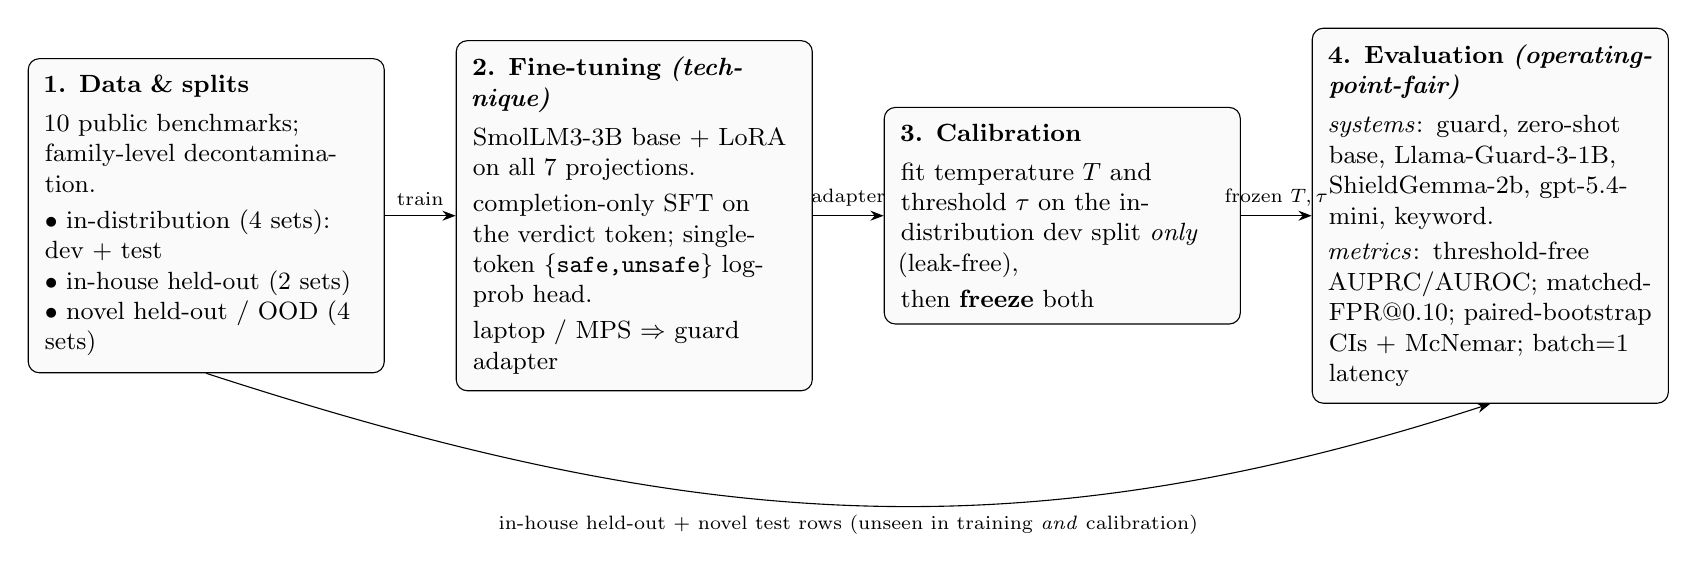
\begin{tikzpicture}[
  >=Stealth, node distance=6mm and 9mm,
  stage/.style={draw, rounded corners, align=left, inner sep=6pt, font=\small, text width=41mm, fill=black!2}
]
  \node[stage] (data) {\textbf{1. Data \& splits}\\[3pt]10 public benchmarks; family-level decontamination.\\[2pt]$\bullet$ in-distribution (4 sets): dev $+$ test\\ $\bullet$ in-house held-out (2 sets)\\ $\bullet$ novel held-out / OOD (4 sets)};
  \node[stage, right=of data] (train) {\textbf{2. Fine-tuning \textit{(technique)}}\\[3pt]SmolLM3-3B base $+$ LoRA on all 7 projections.\\[2pt]completion-only SFT on the verdict token; single-token \texttt{\{safe,unsafe\}} logprob head.\\[2pt]laptop / MPS $\Rightarrow$ guard adapter};
  \node[stage, right=of train] (cal) {\textbf{3. Calibration}\\[3pt]fit temperature $T$ and threshold $\tau$ on the in-distribution dev split \emph{only} (leak-free),\\[2pt]then \textbf{freeze} both};
  \node[stage, right=of cal] (eval) {\textbf{4. Evaluation \textit{(operating-point-fair)}}\\[3pt]\emph{systems}: guard, zero-shot base, Llama-Guard-3-1B, ShieldGemma-2b, gpt-5.4-mini, keyword.\\[2pt]\emph{metrics}: threshold-free AUPRC/AUROC; matched-FPR@0.10; paired-bootstrap CIs $+$ McNemar; batch$=$1 latency};
  \draw[->] (data) -- node[above, font=\scriptsize]{train} (train);
  \draw[->] (train) -- node[above, font=\scriptsize]{adapter} (cal);
  \draw[->] (cal) -- node[above, font=\scriptsize]{frozen $T,\tau$} (eval);
  \draw[->] (data.south) to[out=-18, in=-162] node[below, font=\scriptsize]{in-house held-out $+$ novel test rows (unseen in training \emph{and} calibration)} (eval.south);
\end{tikzpicture}%
}
\caption{End-to-end setup. Only in-distribution \emph{train} rows tune the LoRA guard and only in-distribution \emph{dev} rows calibrate $(T,\tau)$, which are then frozen; every system is scored on the held-out and novel test rows under one operating-point-fair protocol. The zero-shot base is the same network with the LoRA adapter removed. Hyperparameters: \Cref{tab:lora}; calibrated values: \Cref{tab:calibration}; results: \S\ref{sec:results}.}
\label{fig:pipeline}
\end{figure*}

\subsection{Guard formulation: a single-token logprob head}

The guard treats safety classification as a single next-token prediction. A prompt to be screened is wrapped in a fixed instruction template and the model is asked to emit a one-word verdict, \texttt{safe} or \texttt{unsafe}. Rather than sampling text, we read the logits at the final position and restrict attention to the two verdict tokens. Let $z_{\text{safe}}$ and $z_{\text{unsafe}}$ be those logits; the guard score is a temperature-scaled two-way softmax
\begin{equation}
P(\text{unsafe}) = \frac{\exp(z_{\text{unsafe}}/T)}{\exp(z_{\text{safe}}/T) + \exp(z_{\text{unsafe}}/T)}.
\end{equation}
A single forward pass yields the score (\Cref{fig:logprob-head}) --- no autoregressive decoding, no multi-token or chain-of-thought generation. This keeps inference cheap and makes the guard a proper threshold-free scorer, so it can be summarized by AUPRC/AUROC in addition to a hard verdict. A prompt is flagged \texttt{unsafe} when $P(\text{unsafe}) \ge \tau$ for a fixed decision threshold $\tau$.

\begin{figure}[t]
\centering
\resizebox{\columnwidth}{!}{%
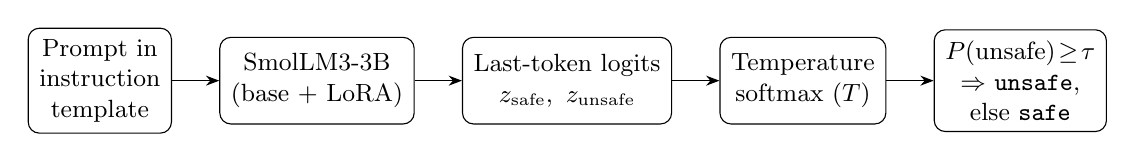
\begin{tikzpicture}[
  >=Stealth,
  node distance=6mm,
  box/.style={draw, rounded corners, align=center, minimum height=11mm, inner sep=4pt, font=\small}
]
  \node[box] (p) {Prompt in\\instruction\\template};
  \node[box, right=of p] (m) {SmolLM3-3B\\(base + LoRA)};
  \node[box, right=of m] (l) {Last-token logits\\$z_{\text{safe}},\ z_{\text{unsafe}}$};
  \node[box, right=of l] (s) {Temperature\\softmax ($T$)};
  \node[box, right=of s] (o) {$P(\text{unsafe})\!\ge\!\tau$\\$\Rightarrow$ \texttt{unsafe},\\else \texttt{safe}};
  \draw[->] (p) -- (m);
  \draw[->] (m) -- (l);
  \draw[->] (l) -- (s);
  \draw[->] (s) -- (o);
\end{tikzpicture}%
}
\caption{The single-token logprob head. A prompt is wrapped in a fixed instruction template and passed once through the LoRA-adapted SmolLM3-3B; the last-position logits over \texttt{\{safe, unsafe\}} are turned into $P(\text{unsafe})$ by a temperature-scaled two-way softmax, and the prompt is flagged when $P(\text{unsafe}) \ge \tau$.}
\label{fig:logprob-head}
\end{figure}

\subsection{Calibration}

The temperature $T$ (temperature scaling \cite{guo2017calibration}) and threshold $\tau$ are the only post-training free parameters, and both are fit exclusively on an \textbf{in-distribution dev split} drawn from the four in-distribution benchmarks (BeaverTails, ToxicChat, Prompt Injections, Jailbreak Classification). The two in-house held-out benchmarks (JailbreakBench, XSTest) and the four novel benchmarks contribute zero rows to calibration; this is a deliberate correction of an earlier pipeline in which held-out dev rows had leaked into temperature/threshold fitting. The clean, leak-free calibration yields the values in \Cref{tab:calibration}.

\begin{table}[t]
\small
\centering
\caption{Post-training calibration parameters, fit on the in-distribution dev split only.}
\label{tab:calibration}
\begin{tabular}{lr}
\toprule
Parameter & Value \\
\midrule
Temperature $T$ & 2.10 \\
Decision threshold $\tau$ & 0.59 \\
\bottomrule
\end{tabular}
\end{table}

Because $\tau$ is tuned on in-distribution dev data, a single global threshold is structurally in-distribution-optimized; we treat this as a limitation and, for cross-model comparison, additionally report matched-FPR and threshold-free operating points rather than relying on the tuned point alone.

\subsection{LoRA training recipe}

We fine-tune SmolLM3-3B \cite{bakouch2025smollm3} with LoRA adapters \cite{hu2021lora} and a completion-only objective: the loss is computed on the verdict token only, so the model is trained to place probability mass on \texttt{safe}/\texttt{unsafe} at the decision position rather than to reproduce the prompt. Adapters are applied to all seven projection matrices (q, k, v, o, gate, up, down). \Cref{tab:lora} summarizes the recipe.

\begin{table}[t]
\small
\centering
\caption{LoRA fine-tuning recipe for the SmolLM3-3B guard.}
\label{tab:lora}
\begin{tabular}{ll}
\toprule
Setting & Value \\
\midrule
Base model & SmolLM3-3B (instruction-tuned) \\
Adapter & LoRA, rank $r=32$, $\alpha=64$, dropout $0.05$ \\
Target modules & q, k, v, o, gate, up, down \\
Loss & Completion-only, on the verdict token \\
Trainable params & 60.5M (1.93\% of 3.14B) \\
Precision & bf16 \\
Optimizer steps & 300 \\
Wall-clock & \textasciitilde{}71 min \\
Seed & 42 \\
\bottomrule
\end{tabular}
\end{table}

Training ran entirely on a consumer Apple M4 Max laptop (36 GB unified memory, MPS backend, no CUDA), demonstrating that the recipe is reproducible at laptop scale. Because ToxicChat is non-commercial, it is used for evaluation only and is excluded from any released model's training data.

\section{Experimental Setup}
\label{sec:setup}

\subsection{Task and label mapping}

The guard is a binary classifier that emits a single-token verdict, \texttt{safe} or \texttt{unsafe}. We read the logits at the last position, take a softmax over the \texttt{\{safe, unsafe\}} token pair, and treat the resulting $P(\text{unsafe})$ as the decision score. A prompt is labeled \texttt{unsafe} if it should be blocked (harmful content, successful jailbreak/injection, policy-violating request) and \texttt{safe} otherwise; the over-refusal axis contributes benign-but-superficially-risky prompts whose gold label is \texttt{safe}. All evaluations reduce to this one score per row, obtained in a single forward pass.

\subsection{Benchmarks and terminology}

We use three explicitly distinguished pools, and we reserve the word ``held-out'' for two of them:

\begin{itemize}
  \item \textbf{In-distribution (in-dist):} BeaverTails, ToxicChat, Prompt Injections, Jailbreak Classification. Contribute dev rows to calibration plus balanced test rows.
  \item \textbf{In-house held-out:} JailbreakBench, XSTest. Same in-house pool, but test-only --- zero dev/calibration rows.
  \item \textbf{Novel held-out (OOD):} WildGuardTest, WildJailbreak, OR-Bench-Hard, HarmBench. Held out at the source-family level; the guard never trained on them.
\end{itemize}

All splits are class-balanced (matched-n). HarmBench is an all-harmful stress set (no negatives), so it is scored by mean $P(\text{unsafe})$ rather than F1/AUPRC and is \textbf{excluded} from any aggregate AUPRC.

\begin{table*}[t]
\centering
\small
\caption{Benchmarks: source, safety axis, split role, and test statistics. Sources are Hugging Face datasets at \texttt{huggingface.co/datasets/$\langle$source$\rangle$}. ``Test n (uns:safe)'' is the balanced test-split size and its unsafe:safe composition. The four in-distribution and two in-house-held-out sets form the 2{,}018-row in-house pool; the three balanced novel sets total 2{,}020 rows (per-set AUPRC in \Cref{tab:novel-auprc}); HarmBench is 200 all-unsafe rows scored separately.}
\label{tab:benchmarks}
\begin{tabular}{lllll}
\toprule
Benchmark & Source (Hugging Face) & Axis & Split role & Test n (uns:safe) \\
\midrule
BeaverTails~\cite{ji2023beavertails} & \texttt{PKU-Alignment/BeaverTails} & guardrail & in-dist (train/dev/test) & 1{,}041 (513:528) \\
ToxicChat~\cite{lin2023toxicchat} & \texttt{lmsys/toxic-chat} & guardrail & in-dist (train/dev/test) & 401 (199:202) \\
Prompt Injections & \texttt{deepset/prompt-injections} & red-team & in-dist (train/dev/test) & 68 (32:36) \\
Jailbreak Classification & \texttt{jackhhao/jailbreak-classification} & red-team & in-dist (train/dev/test) & 148 (73:75) \\
JailbreakBench~\cite{chao2024jailbreakbench} & \texttt{JailbreakBench/JBB-Behaviors} & red-team & in-house held-out (test only) & 120 (58:62) \\
XSTest~\cite{rottger2024xstest} & \texttt{natolambert/xstest-v2-copy} & over-refusal & in-house held-out (test only) & 240 (123:117) \\
\midrule
WildGuardTest~\cite{han2024wildguard} & \texttt{allenai/wildguardmix} & guardrail & novel / OOD (test only) & balanced \\
WildJailbreak~\cite{jiang2024wildteaming} & \texttt{allenai/wildjailbreak} & red-team & novel / OOD (test only) & balanced \\
OR-Bench-Hard~\cite{cui2024orbench} & \texttt{bench-llm/or-bench} & over-refusal & novel / OOD (test only) & balanced \\
HarmBench~\cite{mazeika2024harmbench} & \texttt{walledai/HarmBench} & red-team & novel / OOD (test only) & 200 (all unsafe) \\
\bottomrule
\end{tabular}
\end{table*}

\textbf{Selection.} We pick established, publicly hosted sets that jointly cover the three safety axes --- \emph{guardrail} (harmful content), \emph{red-team} (jailbreaks / prompt injection), and \emph{over-refusal} (benign-but-superficially-risky) --- and we represent each axis in \emph{both} the in-house and the novel pool, so no axis is judged on a single source. XSTest is the over-refusal probe (its gold label is \texttt{safe}); HarmBench is an all-harmful stress set (no negatives), so it is scored by mean $P(\text{unsafe})$ and excluded from any aggregate AUPRC.

\textbf{Train/dev/test separation (per benchmark).} Only the four \emph{in-distribution} sets contribute training and calibration data: each is split into a train portion (LoRA fine-tuning only), a dev portion (fitting $T$ and $\tau$ only), and a class-balanced test portion; the \textbf{1{,}102} in-distribution dev rows come exclusively from these four (JailbreakBench and XSTest contribute \emph{zero} dev/train rows). The two \emph{in-house-held-out} sets and the four \emph{novel} sets are \textbf{test-only}: the guard never sees them in training or calibration. Novel sets are additionally held out at the \emph{source-family} level (the whole dataset family is excluded from training) with near-duplicate filtering, so held-out evaluation measures transfer rather than memorization. Every test split is class-balanced by matched-$n$ sampling except XSTest (over-refusal, majority \texttt{safe}) and HarmBench (all-unsafe). \Cref{fig:pools} shows the split-and-evaluation flow.

\begin{figure*}[t]
\centering
\resizebox{\textwidth}{!}{%
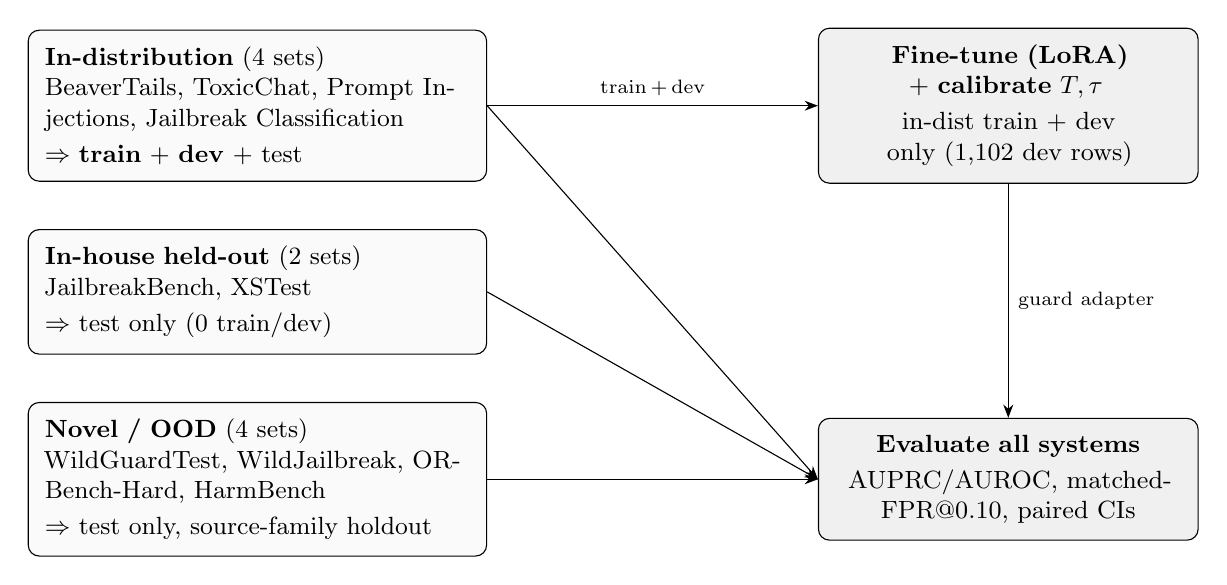
\begin{tikzpicture}[
  >=Stealth,
  pool/.style={draw, rounded corners, align=left, inner sep=6pt, font=\small, text width=54mm, fill=black!2},
  sink/.style={draw, rounded corners, align=center, inner sep=6pt, font=\small, text width=44mm, fill=black!6}
]
  \node[pool] (ind) {\textbf{In-distribution} (4 sets)\\ BeaverTails, ToxicChat, Prompt Injections, Jailbreak Classification\\[2pt] $\Rightarrow$ \textbf{train} $+$ \textbf{dev} $+$ test};
  \node[pool, below=6mm of ind] (iho) {\textbf{In-house held-out} (2 sets)\\ JailbreakBench, XSTest\\[2pt] $\Rightarrow$ test only (0 train/dev)};
  \node[pool, below=6mm of iho] (nov) {\textbf{Novel / OOD} (4 sets)\\ WildGuardTest, WildJailbreak, OR-Bench-Hard, HarmBench\\[2pt] $\Rightarrow$ test only, source-family holdout};
  \node[sink, right=42mm of ind] (train) {\textbf{Fine-tune (LoRA)} $+$ \textbf{calibrate} $T,\tau$\\[2pt] in-dist train $+$ dev only (1{,}102 dev rows)};
  \node[sink, right=42mm of nov] (eval) {\textbf{Evaluate all systems}\\[2pt] AUPRC/AUROC, matched-FPR@0.10, paired CIs};
  \draw[->] (ind.east) -- node[above, font=\scriptsize]{train\,+\,dev} (train.west);
  \draw[->] (ind.east) -- (eval.west);
  \draw[->] (iho.east) -- (eval.west);
  \draw[->] (nov.east) -- (eval.west);
  \draw[->] (train.south) -- node[right, font=\scriptsize]{guard adapter} (eval.north);
\end{tikzpicture}%
}
\caption{Benchmark pools and the train/dev/test separation. Only the four in-distribution sets feed fine-tuning and calibration (train\,+\,dev); the two in-house-held-out and four novel sets are test-only, so held-out and out-of-distribution evaluation measure transfer rather than memorization.}
\label{fig:pools}
\end{figure*}

\subsection{Baselines}

We compare against four systems, each run in its own native regime:

\begin{itemize}
  \item \textbf{gpt-5.4-mini} --- zero-shot classifier prompt at a fixed native decision point (no tunable threshold). On API errors we abstain rather than defaulting to a label (a corrected bug; see \Cref{sec:bugs}).
  \item \textbf{Llama-Guard-3-1B}~\cite{meta2024llamaguard2_3} --- the standard (non-INT4) checkpoint, run with its native chat template, reading the first-token verdict. (The INT4-quantized variant of this 1B model is described separately in~\cite{fedorov2024llamaguard3_1b}; we do not use it.)
  \item \textbf{ShieldGemma-2b} --- its guideline prompt, scored by $P(\text{Yes})$. ShieldGemma is a content-policy / general-guideline guard and is used somewhat outside its designed regime here; it is not an injection detector.
  \item \textbf{Keyword matcher} --- a simple substring/keyword baseline.
\end{itemize}

For a matched comparison we also evaluate an untuned \textbf{base} SmolLM3-3B: zero-shot, with the identical single-token logprob head and no training, on the identical 2,018 test rows as the tuned guard. To keep the comparison fair, the base receives its \emph{own} clean calibration --- a base-specific temperature and threshold ($T{=}7.00,\tau{=}0.51$), fit on the identical in-distribution dev split with the identical NLL-plus-F1 protocol used for the tuned guard --- so each model is read at its own best in-distribution operating point rather than a shared or borrowed threshold. To avoid resting the base-vs-tuned claim on an operating point, we additionally report the base's threshold-free in-house AUPRC (\Cref{sec:base-vs-tuned}).

\subsection{Metrics and which comparisons carry CIs}
\label{sec:metrics}

We report F1 and false-positive rate (FPR) at the operating threshold, and the threshold-free summaries AUPRC and AUROC. Because only our guard receives a dev-tuned threshold while baselines are fixed operating points, we additionally compare all tunable systems at \textbf{matched-FPR@0.10} (threshold chosen so FPR $=0.10$ on the in-distribution dev split) and rely on AUPRC as the fair threshold-free summary. Uncertainty is reported as paired-bootstrap 95\% CIs; pairwise agreement/disagreement between systems is tested with McNemar. Latency is measured at true batch=1 (p50/p90), not batch-amortized.

We are explicit about statistical support: \textbf{only} the guard's pooled/in-house-held-out AUPRC, the guard-vs-Llama-Guard novel aggregate AUPRC, the base-vs-tuned F1 delta, and the guard-vs-GPT $\Delta$F1 carry CIs. Baseline AUPRCs (ShieldGemma, Llama-Guard on the in-house pool) are point estimates. We therefore reserve the word ``decisive'' for the one comparison in which both sides carry CIs and they do not overlap (novel-set guard vs Llama-Guard); elsewhere we say ``leads on point estimates.''

We report several distinct F1 aggregations and define each to prevent conflation:

\begin{itemize}
  \item \textbf{Pooled micro-F1 (0.794):} computed over all 2,018 in-house test rows pooled.
  \item \textbf{Macro-F1, in-dist (0.860):} unweighted mean of per-benchmark F1 over the four in-distribution benchmarks.
  \item \textbf{Macro-F1, in-house held-out (0.827):} unweighted mean of per-benchmark F1 over JailbreakBench and XSTest.
  \item \textbf{Base-vs-tuned aggregate F1 (tuned 0.794, base 0.713):} the base-vs-tuned decomposition (\Cref{sec:base-vs-tuned}) uses these \emph{same} 2,018 pooled rows, so the tuned aggregate equals the pooled micro-F1 above; base and tuned differ only by model (each at its own clean in-distribution calibration), not by row set.
\end{itemize}

\subsection{Decontamination}

Training data is leakage-filtered against the test splits. Our initial pipeline used exact-string-match decontamination. We recommend, and adopt as protocol, source-family holdout plus near-duplicate detection; source-family holdout is what defines and separates the four novel benchmarks, so the guard is evaluated on data from families it never saw during training. We describe near-duplicate detection as the recommended companion to family holdout rather than claiming an exhaustively executed near-duplicate sweep of the release pipeline.

\subsection{Evaluation bugs found and fixed}
\label{sec:bugs}

Building the pipeline surfaced four real bugs in our own first evaluation, each of which we corrected before reporting: (1) a \textbf{calibration leak} in which in-house held-out dev rows had leaked into temperature/threshold fitting --- fixed to in-dist-only calibration ($T=2.10$, $\tau=0.59$); (2) \textbf{batch-amortized latency} (throughput/16) --- replaced with true batch=1 p50/p90; (3) an \textbf{asymmetric threshold advantage} (only our model got a dev-tuned threshold while baselines were fixed points) --- addressed via matched-FPR + threshold-free AUPRC; and (4) a \textbf{GPT error-handling bias} in which API errors defaulted to \texttt{unsafe} (inflating the GPT FPR) --- corrected to \emph{abstain}. We verified this does not affect the reported comparison: an abstention-logged re-score of the in-house GPT baseline found \textbf{zero} API errors in the original run (the fail-closed branch never fired), and it reproduces the tie (GPT FPR $0.321{\to}0.326$; guard\,$-$\,GPT $\Delta$F1 $+0.007$, McNemar $p{=}0.65$).

\subsection{Hardware}

Training and evaluation run on a single consumer Apple M4 Max laptop (36 GB unified memory, MPS backend, no CUDA). Fine-tuning uses LoRA ($r=32$, $\alpha=64$, dropout 0.05, all seven projections) with completion-only loss on the verdict token: 60.5M trainable parameters (1.93\% of 3.14B), bf16, 300 optimizer steps in $\approx$71 minutes, seed 42. Guard inference latency at batch=1 is p50 124 ms / p90 188 ms.

\section{Results}
\label{sec:results}

We report all systems at threshold-free operating points (AUPRC/AUROC) and at a common, conservative operating point (matched-FPR@0.10), with paired-bootstrap 95\% CIs where available. Latency is measured at true batch size 1.

\subsection{Main comparison (in-house pool)}
\label{subsec:main}

Threshold-free AUPRC here is pooled over the \textbf{in-house test rows only} (2,018 rows) --- not over all evaluation rows, since ShieldGemma's novel runs are pending and the novel sets are reported as a separate pool in \Cref{subsec:novel}. Matched-FPR@0.10 fixes every tunable system to the same false-positive rate using a threshold set on the in-distribution dev split. gpt-5.4-mini is reported at its fixed native decision point (no tunable threshold), so it is not directly comparable at matched FPR.

\begin{table*}[t]
\centering
\small
\caption{Main comparison on the in-house pool (2,018 balanced test rows). AUPRC is threshold-free; recall/F1/FPR are reported at matched-FPR@0.10; gpt-5.4-mini is shown at its fixed native decision point. Only the guard carries CIs; baseline AUPRCs are point estimates.}
\label{tab:main-inhouse}
\begin{tabular}{llrrrl}
\toprule
System & AUPRC, in-house pooled [95\% CI] & Recall @FPR 0.10 & F1 @FPR 0.10 & FPR @0.10 & Latency (batch=1) \\
\midrule
Guard (SmolLM3-3B, ours) & \textbf{0.844} [0.825, 0.866] & 0.431 & 0.581 & 0.051 & p50 124 ms / p90 188 ms \\
ShieldGemma-2b & 0.712 & 0.341 & 0.464 & --- & not measured \\
Llama-Guard-3-1B & 0.639 & 0.242 & 0.360 & --- & not measured \\
gpt-5.4-mini (fixed native point) & --- & 0.856 & 0.784 & 0.321 & \textasciitilde{}512 ms (remote API) \\
keyword matcher & --- & 0.096 & 0.168 & --- & not measured \\
\bottomrule
\end{tabular}
\end{table*}

\begin{figure}[t]

\includegraphics[width=\columnwidth]{figures/fig1_inhouse_auprc.pdf}
\caption{Pooled in-house AUPRC (2,018 test rows): the guard (0.844) leads ShieldGemma-2b (0.712) and Llama-Guard-3-1B (0.639) on point estimates.}
\label{fig:inhouse-auprc}
\end{figure}

On pooled in-house AUPRC the guard (0.844) leads ShieldGemma-2b (0.712) and Llama-Guard-3-1B (0.639) on point estimates (the baselines carry no CIs, so we do not assert statistical significance here); see \Cref{fig:inhouse-auprc}. At matched FPR@0.10 all tunable systems are conservative (the guard operates at recall 0.431, FPR 0.051); the guard still leads the other tunable guards on both recall and F1 on point estimates. The guard's in-dist AUPRC is 0.846 and its in-house held-out AUPRC is 0.860 [0.803, 0.909]. At each system's best threshold (Optimal-F1), the guard reaches 0.794, ShieldGemma-2b 0.730, and Llama-Guard-3-1B 0.672 --- the same guard $>$ ShieldGemma $>$ Llama-Guard order, which (like AUPRC) inverts the native-threshold F1 ordering of the two open guards (\Cref{sec:operating-point-fairness}).

\Cref{tab:perbench} breaks the in-house pool down per benchmark: threshold-free AUPRC for every system, plus the base$\to$tuned F1 at each model's own clean in-distribution calibration (the tuned column is also the guard's deployed-point F1). Two patterns stand out. Tuning's F1 gain is concentrated in-distribution and near-flat on the held-out sets (JailbreakBench $+0.012$, XSTest $-0.023$); and on the two held-out sets the \emph{base} already has the higher AUPRC (JailbreakBench 0.967 vs 0.826, XSTest 0.976 vs 0.857), an early sign of the out-of-distribution ranking degradation we quantify in \S\ref{sec:base-vs-tuned}. At the deployed point ($T=2.10$, $\tau=0.59$) this yields macro-F1 0.860 (in-dist) / 0.827 (held-out) and pooled micro-F1 0.794, but the deployed overall FPR is \textbf{0.306} --- at $\tau=0.59$ roughly 31\% of benign in-house prompts are flagged, a genuine deployment concern we revisit in \Cref{sec:limitations}.

\begin{table*}[t]
\centering
\small
\caption{Per-benchmark in-house results. Threshold-free AUPRC (unsafe = positive) for each system, and base$\to$tuned F1 at each model's clean in-distribution calibration. Sets marked $\dagger$ are in-house held-out (test-only, zero train/dev rows); the rest are in-distribution. ``n (uns:safe)'' is the balanced test size. Novel per-set AUPRC is in \Cref{tab:novel-auprc}.}
\label{tab:perbench}
\begin{tabular}{llrrrrr}
\toprule
Benchmark & n (uns:safe) & Guard & Base & Llama-G-3-1B & ShieldGemma-2b & F1 base$\to$tuned \\
\midrule
BeaverTails & 1{,}041 (513:528) & 0.687 & 0.618 & 0.561 & 0.656 & 0.691 $\to$ 0.716 \\
ToxicChat & 401 (199:202) & 0.948 & 0.856 & 0.663 & 0.952 & 0.766 $\to$ 0.915 \\
Prompt Injections & 68 (32:36) & 0.905 & 0.786 & 0.807 & 0.666 & 0.690 $\to$ 0.828 \\
Jailbreak Classification & 148 (73:75) & \textbf{0.999} & 0.451 & 0.662 & 0.824 & 0.339 $\to$ 0.980 \\
JailbreakBench$^\dagger$ & 120 (58:62) & 0.826 & \textbf{0.967} & 0.806 & 0.676 & 0.809 $\to$ 0.821 \\
XSTest$^\dagger$ & 240 (123:117) & 0.857 & \textbf{0.976} & 0.755 & 0.825 & 0.856 $\to$ 0.833 \\
\midrule
\textbf{Pooled (2{,}018)} & (998:1{,}020) & \textbf{0.844} & 0.696 & 0.639 & 0.712 & 0.713 $\to$ 0.794 \\
\bottomrule
\end{tabular}
\end{table*}

\subsection{Novel held-out benchmarks (guard never trained on them)}
\label{subsec:novel}

On the three balanced benchmarks the guard never saw during training, we compare threshold-free AUPRC across the tuned guard, the \emph{zero-shot base}, and Llama-Guard-3-1B (both guard-vs-Llama and base-vs-guard aggregate CIs are non-overlapping).

\begin{table*}[t]
\centering
\small
\caption{Threshold-free AUPRC on the novel held-out benchmarks. The untuned base outranks the tuned guard, which in turn beats Llama-Guard-3-1B; the aggregate is over the three balanced sets (2,020 rows) and excludes HarmBench.}
\label{tab:novel-auprc}
\begin{tabular}{lrrr}
\toprule
Benchmark & Base (zero-shot) AUPRC & Guard (tuned) AUPRC & Llama-Guard-3-1B AUPRC \\
\midrule
wildguardtest & 0.894 & 0.798 & 0.751 \\
wildjailbreak & 0.837 & 0.722 & 0.597 \\
orbench\_hard & 0.940 & 0.845 & 0.750 \\
\midrule
\textbf{Aggregate (2,020 rows)} & \textbf{0.886} [0.870, 0.900] & \textbf{0.781} [0.751, 0.811] & \textbf{0.701} [0.673, 0.733] \\
Aggregate Optimal-F1 & 0.792 & 0.796 & 0.691 \\
\bottomrule
\end{tabular}
\end{table*}

\begin{figure}[t]

\includegraphics[width=\columnwidth]{figures/fig2_novel_auprc.pdf}
\caption{Aggregate AUPRC on the novel held-out benchmarks (2,020 balanced rows): the zero-shot base (0.886) outranks the tuned guard (0.781), which in turn beats Llama-Guard-3-1B (0.701), with non-overlapping 95\% CIs.}
\label{fig:novel-auprc}
\end{figure}

The tuned guard's aggregate AUPRC (0.781 [0.751, 0.811]) exceeds Llama-Guard-3-1B's (0.701 [0.673, 0.733]) with non-overlapping CIs --- a decisive cross-system result. But the \emph{untuned base} ranks higher still (0.886 [0.870, 0.900], disjoint from the tuned guard), while best-threshold F1 is essentially tied across base and guard (0.792 vs 0.796, both above Llama-Guard's 0.691); see \Cref{fig:novel-auprc}. Read together: out-of-distribution the base is the strongest \emph{ranker} (most operating-point-robust), base and tuned guard reach the same \emph{peak} F1, and both beat Llama-Guard. The guard's novel-set lead over Llama-Guard is thus inherited from the base, not produced by LoRA; fine-tuning degrades OOD score ranking (AUPRC) without changing peak achievable F1 (\Cref{sec:base-vs-tuned}).

The aggregate 95\% CIs ([0.751, 0.811] vs [0.673, 0.733]) do not overlap, so this is our one decisive cross-system AUPRC result. The aggregate is over the three balanced novel sets (2,020 rows); \textbf{HarmBench is excluded} from it. On HarmBench (200 all-harmful prompts), mean predicted $P(\text{unsafe})$ is 0.967 for the zero-shot base, 0.780 for the tuned guard, and 0.390 for Llama-Guard-3-1B; because this compares raw probabilities across differently temperature-scaled models it is \emph{suggestive, not decisive} and is not a threshold-free ranking metric (though it echoes the AUPRC ordering base $>$ guard $>$ Llama-Guard). ShieldGemma-2b on the novel benchmarks is \textbf{pending} (Gemma-2 stalls on the throttled MPS laptop); on the in-house held-out set its AUPRC is 0.785 versus the guard's 0.860. We therefore make \textbf{no} ShieldGemma novel-set claim.

\subsection{Frontier comparison: statistical tie and Pareto-style position}
\label{subsec:frontier}

Against gpt-5.4-mini on paired rows, the guard shows no statistically significant F1 difference.

\begin{table}[t]
\centering
\small
\caption{Guard versus gpt-5.4-mini on paired rows: a statistical tie on F1 at roughly 4x lower batch=1 latency.}
\label{tab:frontier}
\begin{tabular}{ll}
\toprule
Comparison (guard vs gpt-5.4-mini) & Value \\
\midrule
$\Delta$F1 (guard $-$ gpt) & $+0.010$ \\
95\% CI & $[-0.006, 0.027]$ \\
McNemar $p$ & 0.20 \\
Guard latency (batch=1) & 124 ms (local M4 Max) \\
gpt-5.4-mini latency & \textasciitilde{}512 ms (remote API) \\
\bottomrule
\end{tabular}
\end{table}

\begin{figure}[t]

\includegraphics[width=\columnwidth]{figures/fig5_pareto.pdf}
\caption{F1 versus single-request (batch=1) latency: the guard sits at parity with gpt-5.4-mini on F1 at roughly 4x lower latency (124 ms vs \textasciitilde{}512 ms per request).}
\label{fig:pareto}
\end{figure}

The F1 difference is not significant (McNemar $p=0.20$; CI spans zero, its lower bound admitting the guard being 0.006 \emph{worse}), so this is a statistical \textbf{tie} with the guard nominally ahead, not an accuracy beat. Two caveats. First, this comparison places the guard at its in-dist-tuned threshold ($\tau=0.59$) against gpt at its fixed native point --- the same per-model-threshold asymmetry we criticize in \Cref{sec:operating-point-fairness}; because gpt exposes no tunable threshold, a matched-FPR comparison is not possible, so the tie is threshold-advantaged in the guard's favor and should be read as such. Second, latency is cross-substrate: 124 ms is local M4 Max inference while \textasciitilde{}512 ms is a remote API round-trip (network plus server-side batching), so ``\textasciitilde{}4x lower latency'' is deployment-realistic but \emph{not} a controlled hardware comparison, and it is a \textbf{guard-vs-gpt claim only} --- Llama-Guard and ShieldGemma latency were not measured. With those caveats, the guard achieves parity accuracy locally at roughly 4x lower batch=1 latency with no API cost: an efficiency win at parity accuracy rather than an accuracy win (\Cref{fig:pareto}).

\section{Analysis}
\label{sec:analysis}

The three analyses below share one message, summarized in \Cref{fig:ranking-flip}: the \emph{same} candidate systems change rank as the evaluation regime changes, so the reported ``best guard'' is a property of the benchmark and operating point as much as of the model.

\begin{figure}[t]
\centering
\resizebox{\columnwidth}{!}{%
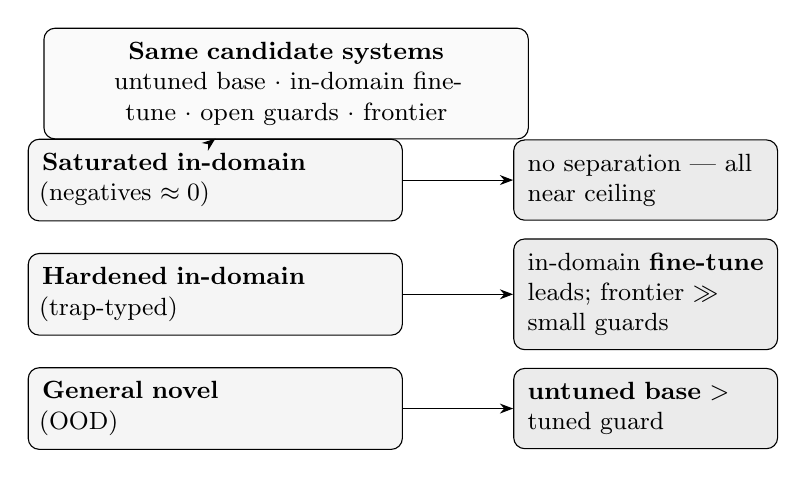
\begin{tikzpicture}[
  >=Stealth,
  cand/.style={draw, rounded corners, align=center, inner sep=5pt, font=\small, text width=58mm, fill=black!2},
  regime/.style={draw, rounded corners, align=left, inner sep=5pt, font=\small, text width=44mm, fill=black!4},
  win/.style={draw, rounded corners, align=left, inner sep=5pt, font=\small, text width=30mm, fill=black!8}
]
  \node[cand] (c) {\textbf{Same candidate systems}\\ untuned base $\cdot$ in-domain fine-tune $\cdot$ open guards $\cdot$ frontier};
  \node[regime, below=7mm of c.west, anchor=north west, xshift=-2mm] (r1) {\textbf{Saturated in-domain}\\ (negatives $\approx 0$)};
  \node[regime, below=4mm of r1] (r2) {\textbf{Hardened in-domain}\\ (trap-typed)};
  \node[regime, below=4mm of r2] (r3) {\textbf{General novel}\\ (OOD)};
  \node[win, right=14mm of r1] (w1) {no separation --- all near ceiling};
  \node[win, right=14mm of r2] (w2) {in-domain \textbf{fine-tune} leads; frontier $\gg$ small guards};
  \node[win, right=14mm of r3] (w3) {\textbf{untuned base} $>$ tuned guard};
  \draw[->] (c) -- (r1.north);
  \draw[->] (r1) -- (w1);
  \draw[->] (r2) -- (w2);
  \draw[->] (r3) -- (w3);
\end{tikzpicture}%
}
\caption{The benchmark chooses the winner. The identical systems yield a different verdict per regime: a saturated benchmark separates nobody; a hardened in-domain rebuild is led by the in-domain fine-tune, with a frontier model far ahead of every small guard; and on general out-of-distribution benchmarks the untuned base outranks the tuned guard (\S\ref{sec:base-vs-tuned}, \S\ref{sec:mortgage-casestudy}).}
\label{fig:ranking-flip}
\end{figure}

\subsection{Base-vs-tuned decomposition: PEFT specializes in-distribution and degrades OOD ranking}
\label{sec:base-vs-tuned}

We isolate the contribution of parameter-efficient fine-tuning by evaluating the base SmolLM3-3B model zero-shot with the identical single-token logprob head (no training), on the identical paired rows.

Two findings stand out. First, the \emph{untuned} base is already a competent safety classifier by F1: its zero-shot F1 of 0.713 exceeds the zero-shot F1 of both purpose-built open guards --- Llama-Guard-3-1B (0.673) and ShieldGemma-2b (0.424). Consistent with our own Contribution \#1, this is an \textbf{F1-at-operating-point} comparison, so we also measured the base's threshold-free in-house AUPRC: 0.696 [0.666, 0.730]. This \emph{confirms} the caution we flagged rather than overturning it --- under AUPRC the base (0.696) falls \emph{between} Llama-Guard-3-1B (0.639) and ShieldGemma-2b (0.712), so the base's by-F1 lead over ShieldGemma does \textbf{not} survive the threshold-free test in-house. The threshold-free ``base is a strong guard'' claim holds only \emph{out-of-distribution}: on the four novel benchmarks the base's AUPRC (0.886) beats every system we could measure there (Llama-Guard-3-1B 0.701; see \Cref{subsec:novel}).

Second, LoRA adds a real but \emph{localized} gain: aggregate F1 on the identical 2,018 paired rows (each model at its own clean in-distribution calibration) rises from 0.713 to 0.794 (delta $+0.081$, 95\% CI [0.062, 0.100], McNemar $p < 1\mathrm{e}{-4}$). Decomposing this delta per benchmark shows it is concentrated almost entirely in the in-distribution axes and is essentially flat on the two in-house held-out benchmarks (JailbreakBench $+0.012$, XSTest $-0.023$; macro $-0.005$). The threshold-free picture is symmetric and sharper: tuning \emph{raises} the guard's in-house AUPRC from the base's 0.696 to 0.844, yet \emph{lowers} its novel-set AUPRC from the base's 0.886 to 0.781 --- LoRA specializes the ranker to the in-distribution regime at the cost of out-of-distribution ranking.

The base's in-house shortfall is concentrated, not uniform. Per-benchmark, the base's low in-house AUPRC (0.696) comes almost entirely from BeaverTails --- where the zero-shot base over-flags edgy-but-benign prompts (AUPRC 0.618, and this set is 52\% of the pool) --- and from jailbreak\_classification, which the zero-shot base \emph{inverts} (0.451, below chance); on the other four in-house benchmarks and all three novel sets the base already ranks well (0.79--0.98). Tuning's in-house AUPRC lift is therefore mostly the repair of these two weak spots (jailbreak\_classification $0.451 \to 0.999$) plus improved score comparability across benchmarks --- the pooled-versus-macro-mean gap shrinks from 0.080 (base 0.696 vs 0.776) to 0.026 (tuned 0.844 vs 0.870) --- rather than a broad gain in discrimination. This also explains the base's counterintuitive in-house-below-novel ordering: it is a benchmark-composition effect (the in-house pool contains the base's two blind spots; the novel pool does not), not evidence that the base generalizes better to unseen data than to seen data.

\begin{table*}[t]
\small
\centering
\caption{Per-benchmark base-vs-tuned F1 decomposition on the identical 2,018 in-house test rows, each model at its own clean in-distribution calibration (tuned $T{=}2.10,\tau{=}0.59$; base $T{=}7.00,\tau{=}0.51$). Positive deltas are concentrated in-distribution; the two in-house held-out benchmarks move only marginally (macro $-0.005$).}
\label{tab:base-vs-tuned}
\begin{tabular}{llrrr}
\toprule
Benchmark & Split & Base F1 & Tuned F1 & Delta \\
\midrule
jailbreak\_classification & in-dist & 0.339 & 0.980 & $+0.641$ \\
toxicchat & in-dist & 0.766 & 0.915 & $+0.150$ \\
prompt\_injections & in-dist & 0.690 & 0.828 & $+0.138$ \\
beavertails & in-dist & 0.691 & 0.716 & $+0.024$ \\
jailbreakbench & in-house held-out & 0.809 & 0.821 & $+0.012$ \\
xstest & in-house held-out & 0.856 & 0.833 & $-0.023$ \\
\midrule
\textbf{Aggregate (paired rows)} & & \textbf{0.713} & \textbf{0.794} & \textbf{$+0.081$ [0.062, 0.100]} \\
\bottomrule
\end{tabular}
\end{table*}

\begin{figure}[t]

\includegraphics[width=\columnwidth]{figures/fig4_base_vs_tuned.pdf}
\caption{Per-benchmark base $\to$ tuned F1 delta. LoRA gains are positive in-distribution and flat-to-negative on the in-house held-out benchmarks.}
\label{fig:base-vs-tuned}
\end{figure}

The pattern is unambiguous within its scope: every large positive delta is in-distribution (the extreme case, jailbreak\_classification, $+0.641$, is a task the base essentially could not do), while the two in-house held-out benchmarks barely move (JailbreakBench $+0.012$, XSTest $-0.023$; macro $-0.005$), including a small regression on the over-refusal probe (XSTest). \Cref{fig:base-vs-tuned} visualizes this split. LoRA specializes the guard to the training distribution's label conventions and formatting; on the two in-house held-out benchmarks it does not measurably improve --- and on over-refusal can mildly degrade --- generalization.

We have now measured the base on the four novel benchmarks, which \textbf{confirms and sharpens} this claim. Out-of-distribution, the \emph{untuned} base ranks higher than the tuned guard (aggregate AUPRC 0.886 [0.870, 0.900] vs 0.781 [0.751, 0.811], non-overlapping CIs), while both reach essentially the same best-threshold F1 (0.792 vs 0.796). Fine-tuning therefore does not merely fail to help OOD --- it \emph{degrades the guard's OOD score ranking / operating-point robustness}: a lower AUPRC means a worse precision--recall trade-off across thresholds, even though a per-distribution re-tuned threshold would recover the same peak F1 (a re-tuning that is, by definition, unavailable on unseen data). This resolves the earlier tension between Contribution \#2 (tuning does not improve --- and on OOD ranking actively harms --- generalization) and Contribution \#3 (the tuned guard still beats Llama-Guard on novel data): the guard's novel-set lead is \emph{inherited from the base}, not produced by LoRA, and the base in fact beats Llama-Guard by an even larger margin.

This is the constructive complement to prior reports that fine-tuning can \emph{destroy} safety alignment: here tuning ``works,'' yet the measurable gain is memorization of the in-distribution operating regime rather than demonstrated transferable safety competence.

\subsection{Case study: a saturated domain benchmark and its hardened rebuild}
\label{sec:mortgage-casestudy}

The base-vs-tuned finding above is not specific to our novel sets: the winner also moves when we control a benchmark's difficulty directly. Take a domain guard task --- mortgage fair-lending, compliance, and security-misuse prompts. The obvious benchmark is \emph{saturated}: the flag and allow classes are lexically separable (overt violations vs.\ clean textbook questions) and the negatives sit near probability zero, so a floor threshold trivially divides them and every system --- base, in-domain fine-tune, and open guards alike --- scores near the ceiling and is statistically indistinguishable. A saturated set cannot rank guards, so we replace it with a hardened one.

The hardened set\footnote{Released in the artifact bundle as \texttt{guard\_benchmark\_hard.jsonl} (334 items) and scored by \texttt{eval\_mortgage\_hard.py}; the saturated legacy set \texttt{guard\_benchmark.jsonl} is released alongside. Full paths are in the repository README.} contains 334 trap-typed items (195 unsafe / 139 safe; 284 \emph{very-hard} and 50 \emph{borderline}; loan-officer and consumer personas) engineered to defeat surface cues (\Cref{tab:hardcomp}). It mixes disguised \emph{positives} --- minimal-pair twins, euphemism, coded-proxy, buried instruction-injection, dual-use, and multi-turn setups --- with hard \emph{negatives}: benign prompts that look risky, such as fair-lending education questions, legitimate business-justified underwriting, and over-refusal bait. The set has no train/dev split, so we report operating-point-independent AUPRC and Optimal-F1 as the fair primary, plus accuracy, recall, precision, and FPR at each system's own best-F1 point (gpt-5.4-mini at its native point).

\begin{table}[t]
\small
\centering
\caption{Composition of the hardened mortgage set (334 items). ``Trap type'' is the surface cue an item is built to defeat; \emph{hard\_negative} items are benign prompts that superficially resemble violations. Also: 195 unsafe / 139 safe; difficulty very-hard 284 / borderline 50; categories safe 139, security-misuse 89, fair-lending 65, compliance 41.}
\label{tab:hardcomp}
\begin{tabular}{lr}
\toprule
Trap type & n \\
\midrule
hard\_negative (benign, looks risky) & 75 \\
minimal\_pair & 60 \\
euphemism & 52 \\
business\_justified & 45 \\
buried\_injection & 39 \\
over\_refusal\_bait & 20 \\
dual\_use & 15 \\
multi\_turn & 15 \\
coded\_proxy & 13 \\
\bottomrule
\end{tabular}
\end{table}

Three things follow (\Cref{tab:mortgage-casestudy}). First, the hardened set \textbf{de-saturates} the comparison: where the saturated version left every system near the ceiling, here threshold-free AUPRC spreads from 0.82 to 0.92 and accuracy from 0.65 to 0.95. Second, the difficulty is \textbf{over-blocking, not misses}: every small guard keeps high recall on the disguised positives (0.93--0.95; minimal-pair and coded-proxy catch-rates $\approx$1.0) but pays a steep false-positive rate on the hard negatives (base 0.53, general-safety guard 0.74, mortgage-SFT 0.27). The frontier gpt-5.4-mini sits at FPR 0.065 for comparable recall (0.96). We stress this last comparison is \emph{not} a matched operating point --- each local guard is read at its own best-F1 threshold and gpt at its fixed native point --- so it is suggestive of a small-guard-vs-frontier capability gap rather than a controlled one; the threshold-free AUPRC below is the claim we lean on. Third, the \textbf{winner is benchmark-dependent} (on the fair, threshold-free AUPRC): the in-domain mortgage-SFT --- indistinguishable on the saturated set --- has the highest AUPRC here (0.924), ahead of the untuned base (0.892; the gap is within overlapping CIs) and clearly ahead of the general-safety guard (0.824). This is the \emph{opposite} in-domain-tuning verdict from the general novel benchmarks (\S\ref{sec:base-vs-tuned}), where the untuned base outranks the tuned guard --- so whether in-domain fine-tuning helps depends on whether the hard test is in-domain or general OOD.

\begin{table*}[t]
\centering
\small
\caption{Results on the hardened mortgage benchmark (334 items). AUPRC and Optimal-F1 are threshold-free / operating-point-independent (fair primary); accuracy, recall, precision, and FPR are at each system's own best-F1 point, with gpt-5.4-mini at its native decision point. Every small guard over-blocks the hard negatives (FPR 0.27--0.74) where the frontier holds 0.065; the in-domain fine-tune is the strongest small guard.}
\label{tab:mortgage-casestudy}
\begin{tabular}{lrrrrrr}
\toprule
System & AUPRC [95\% CI] & Opt-F1 & Accuracy & Recall & Precision & FPR \\
\midrule
Base (zero-shot SmolLM3-3B) & 0.892 [0.854, 0.925] & 0.819 & 0.754 & 0.954 & 0.718 & 0.525 \\
Mortgage-SFT (in-domain LoRA) & 0.924 [0.849, 0.946] & 0.885 & 0.856 & 0.949 & 0.830 & 0.273 \\
General-safety guard (ours) & 0.824 [0.774, 0.873] & 0.756 & 0.650 & 0.928 & 0.637 & 0.741 \\
gpt-5.4-mini (frontier ceiling) & --- & --- & \textbf{0.949} & \textbf{0.959} & \textbf{0.954} & \textbf{0.065} \\
\bottomrule
\end{tabular}
\end{table*}

We present this as a case study, not a headline benchmark: the hardened set is seed-scale (334 items) and single-annotator, and because every system keeps high recall the discriminating signal lives in AUPRC and FPR rather than recall. Absolute magnitudes will move under broader adjudication; the robust reading is comparative --- the de-saturation, the small-guard-vs-frontier FPR gap, and the benchmark-dependent fine-tuning verdict (in-domain tuning leads \emph{here} but the untuned base leads on general OOD) --- all instances of the benchmark choosing the winner.

\subsection{Operating-point fairness: rankings depend on the threshold}
\label{sec:operating-point-fairness}

Guard rankings shift substantially with the decision threshold, so any comparison that reads F1 at each model's \emph{native} operating point conflates classifier quality with operating-point choice. Concretely, at native thresholds Llama-Guard-3-1B posts a higher F1 than ShieldGemma-2b (0.673 vs 0.424), but this ordering \textbf{reverses} under both threshold-free AUPRC (0.639 vs 0.712) and best-threshold Optimal-F1 (0.672 vs 0.730): a ranking flip that is purely an artifact of where each model's alarm is set. \Cref{fig:operating-point-flip} shows this flip. Only our model received a dev-tuned threshold; the baselines were fixed points. We therefore report both threshold-free AUPRC and a matched-FPR comparison, with paired-bootstrap CIs where available.

\begin{figure}[t]

\includegraphics[width=\columnwidth]{figures/fig3_operating_point_flip.pdf}
\caption{ShieldGemma-2b vs Llama-Guard-3-1B under native-threshold F1, threshold-free AUPRC, and matched-FPR@0.10: the native-F1 ranking inverts under both operating-point-fair metrics.}
\label{fig:operating-point-flip}
\end{figure}

Threshold-free, the guard leads the open guards across every in-house pooling, on point estimates (baseline AUPRCs carry no CIs):

\begin{table}[t]
\small
\centering
\caption{Threshold-free AUPRC across in-house poolings. The guard leads on point estimates; only the guard carries CIs.}
\label{tab:auprc-poolings}
\begin{tabular}{lrrr}
\toprule
System & \makecell[r]{AUPRC\\in-house pooled} & \makecell[r]{AUPRC\\in-dist} & \makecell[r]{AUPRC\\in-house held-out} \\
\midrule
Guard & 0.844 [0.825, 0.866] & 0.846 & 0.860 [0.803, 0.909] \\
ShieldGemma-2b & 0.712 & 0.702 & 0.785 \\
Llama-Guard-3-1B & 0.639 & 0.610 & 0.762 \\
\bottomrule
\end{tabular}
\end{table}

At a conservative operating point (each tunable system's threshold set so its FPR$=$0.10 on the in-distribution \emph{dev} split), the ranking is preserved on point estimates but all systems are pushed to low recall. The realized \emph{test} FPRs are not identical --- guard 0.051, Llama-Guard-3-1B 0.101, ShieldGemma-2b 0.125 --- so ``matched-FPR@0.10'' is matched on the \emph{dev} split; on the test pool the guard is in fact held to a \emph{stricter} operating point than the baselines, which disadvantages rather than flatters it:

\begin{table}[t]
\small
\centering
\caption{Dev-matched FPR$=$0.10 operating point (threshold set so FPR$=$0.10 on the in-distribution dev split; realized \emph{test} FPRs differ and are shown in the FPR column). gpt-5.4-mini and the keyword matcher are at their fixed native points.}
\label{tab:matched-fpr}
\begin{tabular}{lrrr}
\toprule
System & Recall & F1 & FPR \\
\midrule
Guard & 0.431 & 0.581 & 0.051 \\
ShieldGemma-2b & 0.341 & 0.464 & 0.125 \\
Llama-Guard-3-1B & 0.242 & 0.360 & 0.101 \\
keyword matcher & 0.096 & 0.168 & 0.047 \\
gpt-5.4-mini (fixed native point) & 0.856 & 0.784 & 0.321 \\
\bottomrule
\end{tabular}
\end{table}

Why native-threshold F1 comparisons mislead: gpt-5.4-mini's native point trades a high FPR (0.321) for high recall (0.856), producing an F1 of 0.784 that is not comparable to a guard evaluated at FPR 0.051. Conversely, the matched-FPR@0.10 constraint makes \emph{every} system conservative --- the guard's recall there is only 0.431 --- so matched-FPR alone understates absolute capability. The two views are complementary: matched-FPR fixes the confound of who got to tune a threshold, and AUPRC is the threshold-free summary that removes operating-point choice entirely. Read together they give a consistent picture on point estimates --- guard $>$ ShieldGemma-2b $>$ Llama-Guard-3-1B --- with the one formally supported (non-overlapping-CI) statement being the guard's novel-set lead over Llama-Guard (see \Cref{subsec:novel}).

\section{Limitations}
\label{sec:limitations}

We frame these results as a measurement and controlled study, not a state-of-the-art claim. Several caveats bound their interpretation.

\textbf{Deployed operating point over-blocks.} At the deployed point ($T=2.10$, $\tau=0.59$) the guard's overall FPR is 0.306 --- roughly 31\% of benign in-house prompts are flagged \texttt{unsafe}. This is a real deployment concern: a global $\tau$ tuned for balanced F1 on in-dist dev data is too aggressive for many production settings, which would need a higher, application-specific threshold (trading recall for fewer false positives). We report the deployed point for transparency, but we do not recommend $\tau=0.59$ as an out-of-the-box safe default.

\textbf{Operating point and matched-FPR conservatism.} A single global threshold is structurally in-distribution-optimized, and guard rankings depend heavily on the decision threshold. Our matched-FPR@0.10 comparison forces all systems into a conservative regime: at that operating point the guard's recall is only 0.431 (F1 0.581, FPR 0.051). We therefore treat threshold-free AUPRC as the fair primary summary and matched-FPR as a secondary, deliberately strict view.

\textbf{Statistical support is uneven.} Only four comparisons carry CIs (guard pooled/in-house-held-out AUPRC, guard-vs-Llama novel aggregate, base-vs-tuned F1 delta, guard-vs-GPT $\Delta$F1). Baseline AUPRCs are point estimates, so the pooled/in-dist ``leads'' and the matched-FPR ranking are point-estimate claims, not significance tests. We reserve ``decisive'' for the single non-overlapping-CI result (novel guard vs Llama-Guard).

\textbf{GPT is a tie, not a beat, and threshold-advantaged.} Against gpt-5.4-mini the guard shows no significant F1 difference:

\begin{table}[t]
\small
\centering
\caption{Guard vs gpt-5.4-mini: paired F1 comparison.}
\label{tab:guard-vs-gpt}
\begin{tabular}{lrrr}
\toprule
Comparison & $\Delta$F1 & 95\% CI & McNemar \\
\midrule
guard vs gpt-5.4-mini & +0.010 & [-0.006, 0.027] & p=0.20 \\
\bottomrule
\end{tabular}
\end{table}

The guard is nominally ahead but the difference is not significant, and the comparison uses the guard's dev-tuned threshold against gpt's fixed native point (gpt exposes no tunable threshold, so a matched-FPR comparison is impossible). The advantage over GPT is an efficiency one (local, \textasciitilde{}4$\times$ lower batch=1 latency: 124 ms vs \textasciitilde{}512 ms per request, no API cost), not an accuracy win, and the latency figure is cross-substrate (local inference vs remote API), not a controlled hardware benchmark.

\textbf{Novel-set win is inherited, not tuned.} We ran the base SmolLM3-3B on the four novel benchmarks: it \emph{outranks} the tuned guard OOD (aggregate AUPRC 0.886 [0.870, 0.900] vs 0.781), so the guard's novel-set advantage over Llama-Guard reflects inherited base competence, and LoRA in fact degrades OOD ranking (\Cref{sec:base-vs-tuned}). This result is anchored on threshold-free AUPRC and best-threshold Optimal-F1 (both operating-point-independent), so it does not depend on any calibration choice. The in-house base-vs-tuned F1 delta uses a base-specific clean calibration ($T{=}7.00,\tau{=}0.51$) fit on the same in-distribution dev split and protocol as the tuned guard --- so each model is read at its own best in-distribution operating point --- and we additionally report the base's threshold-free in-house AUPRC (0.696), which places it between the two open guards and confirms the in-house base-competence claim is by F1 only (\Cref{sec:base-vs-tuned}).

\textbf{Generalization claim rests on two benchmarks.} The ``PEFT specializes but does not improve generalization'' finding is evidenced by only the two in-house held-out benchmarks (JailbreakBench, XSTest); it is not a broad OOD-generalization result.

\textbf{ShieldGemma out-of-regime and pending on the novel set.} ShieldGemma-2b is designed for content-policy / general-guideline moderation and is not an injection detector; using it across our red-team axes is somewhat out of its designed regime, so its numbers may understate its intended performance. On the in-house held-out set its AUPRC is 0.785 vs the guard's 0.860. Its results on the four novel held-out benchmarks are \textbf{pending} (Gemma-2 stalls on the throttled MPS laptop) and are not reported here; we make no ShieldGemma novel-set claim.

\textbf{HarmBench metric is calibration-dependent.} The HarmBench comparison (mean $P(\text{unsafe})$ 0.780 vs 0.390) compares raw probabilities across differently temperature-scaled models; it is suggestive, not decisive, and HarmBench is excluded from the aggregate AUPRC.

\textbf{Dataset licensing.} ToxicChat is non-commercial; it is eval-only for any released model and cannot be used to train a distributed guard.

\textbf{Sample sizes and CIs.} Some benchmarks have small n and correspondingly wide CIs, so per-benchmark point estimates should be read with their intervals (e.g., in-house held-out AUPRC 0.860 [0.803, 0.909]).

\textbf{Decontamination scope.} We adopt source-family holdout to define the novel benchmarks and recommend near-duplicate detection as the companion protocol; we do not claim an exhaustive near-duplicate sweep of the entire release pipeline.

\textbf{Scope of the guard and evaluation.} The guard emits a single-token verdict from one forward pass; we do not evaluate a multi-token or reasoning-style guard, and adversarial-robustness evaluation (e.g., against adaptive attacks) is future work.

\section{Conclusion}

We presented a binary \emph{input-prompt} safety guard --- the prompt-classification component of the \textsc{agent-bouncer} project --- obtained by parameter-efficient fine-tuning of SmolLM3-3B on a single consumer laptop (Apple M4 Max, MPS, no CUDA; \textasciitilde{}71 min / 300 steps; 60.5M trainable params, 1.93\% of 3.14B). The guard emits a single-token verdict in one forward pass at batch=1 p50 124 ms / p90 188 ms. Our central finding is a measurement one: guard rankings depend heavily on the decision threshold, so we evaluate at matched FPR, with threshold-free AUPRC/AUROC, paired-bootstrap 95\% CIs, and McNemar tests. Building the pipeline surfaced and let us fix real evaluation bugs (calibration leak, batch-amortized latency, per-model-only threshold tuning, GPT error-to-``unsafe'' default, exact-string decontamination).

Under this protocol the results are modest and specific rather than sweeping:

\begin{table*}[t]
\centering
\small
\caption{Summary of the guard's headline comparisons under the operating-point-fair protocol. CIs are 95\% paired-bootstrap intervals; baseline point estimates without CIs are reported as such.}
\label{tab:conclusion-summary}
\begin{tabular}{llll}
\toprule
Comparison & Metric & Guard & Baseline \\
\midrule
vs Llama-Guard-3-1B (novel held-out) & aggregate AUPRC & 0.781 [0.751, 0.811] & 0.701 [0.673, 0.733] \\
vs Llama-Guard-3-1B (in-house pooled) & AUPRC (point est.) & 0.844 [0.825, 0.866] & 0.639 \\
vs ShieldGemma-2b (in-house pooled) & AUPRC (point est.) & 0.844 & 0.712 \\
vs gpt-5.4-mini (paired) & $\Delta$F1 & +0.010 [-0.006, 0.027], McNemar $p=0.20$ & --- \\
vs gpt-5.4-mini & latency (batch=1) & 124 ms (local) & \textasciitilde{}512 ms (remote API) \\
\bottomrule
\end{tabular}
\end{table*}

On threshold-free AUPRC the guard surpasses Llama-Guard-3-1B decisively --- the only non-overlapping-CI cross-system result, and it holds on the four novel held-out benchmarks --- and it exceeds ShieldGemma-2b on the in-house pooled / in-dist / in-house-held-out sets on point estimates (ShieldGemma's novel runs are pending). It is a statistical tie with gpt-5.4-mini on F1 at \textasciitilde{}4x lower batch=1 latency and no API cost: an efficiency win at parity accuracy, not an accuracy beat.

Our base-vs-tuned decomposition tempers the fine-tuning narrative (numbers in \Cref{tab:related-base-vs-tuned,tab:novel-auprc}). The zero-shot base is already a competent classifier, and LoRA's gains are almost entirely in-distribution: the two in-house held-out benchmarks barely move, and on the four novel benchmarks the \emph{untuned} base actually outranks the tuned guard (aggregate AUPRC 0.886 vs 0.781, disjoint CIs) at tied peak F1. The guard's out-of-distribution lead is therefore inherited base competence, and tuning \emph{degrades} out-of-distribution ranking rather than improving generalization. The mortgage case study (\S\ref{sec:mortgage-casestudy}) makes the point in a domain: a saturated benchmark ranks every system near the ceiling, while a hardened, trap-typed rebuild de-saturates the field and exposes a small-guard-vs-frontier over-blocking gap (benign FPR 0.27--0.74 vs.\ 0.065) --- and the fine-tuning verdict flips (in-domain tuning leads there, the untuned base leads on general OOD). The recurring lesson is that a guard's apparent quality is inseparable from the operating point and the benchmark it is measured on.

We are candid about scope. Matched-FPR@0.10 makes every system conservative (guard recall 0.431 there), so AUPRC is our fairest summary, and the \emph{deployed} point over-blocks (FPR 0.306). A single global threshold is structurally in-distribution-optimized. ShieldGemma is exercised somewhat outside its designed content-policy regime and its novel-benchmark AUPRC is still pending. Some benchmark n are small (wide CIs). The guard is single-token with no reasoning or adversarial-robustness evaluation, and ToxicChat is eval-only under its non-commercial terms.

\subsection{Future Work}\label{sec:future}

\begin{itemize}
  \item \textbf{Specializing without sacrificing OOD robustness.} Since fine-tuning specialized in-distribution but \emph{degraded} the base's OOD score ranking (\Cref{sec:base-vs-tuned}), a central direction is training recipes --- broad, family-decontaminated data plus regularization --- that add in-distribution competence \emph{without} losing the untuned base's operating-point robustness on unseen distributions.
  \item \textbf{Broad-data training as the generalization lever.} Since tuning specialized in-distribution without improving the in-house held-out F1, the most promising direction is scaling and diversifying training data (source-family coverage, near-duplicate-filtered) to test whether generalization, not just in-distribution fit, can be trained in.
  \item \textbf{Controlled objective comparison.} A like-for-like head-to-head of SFT vs DPO~\cite{rafailov2023dpo} vs IPO~\cite{azar2023ipo} vs KTO~\cite{ethayarajh2024kto} vs ORPO~\cite{hong2024orpo} (and single-token GRPO~\cite{shao2024deepseekmath} vs PPO~\cite{schulman2017ppo}) under identical data, splits, and calibration, to isolate the effect of the learning objective on both in-distribution specialization and held-out transfer.
  \item \textbf{Hardened, expert-labeled benchmarks.} The mortgage case study (\Cref{sec:mortgage-casestudy}) used a seed-scale, single-annotator hardened set; expert re-adjudication, scaling, and applying the same saturated-vs-hardened rebuild across domains would turn the observations --- de-saturation and the small-guard-vs-frontier over-blocking gap --- from a case study into a headline result, and provide a benchmark whose difficulty is calibrated to model capability.
  \item \textbf{Adversarial robustness.} Evaluation and hardening against paraphrase, obfuscation, and prompt-level attacks, which our current single-token guard does not measure.
  \item \textbf{Agent surfaces (the namesake, not yet evaluated).} Extending the guard beyond input prompts to tool-call arguments, tool outputs, and model responses --- the surfaces that motivate the \textsc{agent-bouncer} name but that this paper does \emph{not} evaluate. This is the highest-value next step and the most direct way to make the ``agent'' framing empirical rather than aspirational.
  \item \textbf{Completing the baseline matrix.} Resolving the pending ShieldGemma-2b runs on the novel held-out benchmarks, and measuring open-guard latency, for a complete threshold-free and efficiency comparison.
\end{itemize}

Code, calibration, and the full evaluation protocol are released as open code --- the evaluation scripts plus a single orchestrating reproduction notebook (\texttt{paper\_reproduction.ipynb}) --- to support reproduction at laptop scale.

\emph{Baseline note: \texttt{gpt-5.4-mini} is a hosted commercial API model with no public paper or model card; we cite it as an API baseline rather than a bibliographic reference.}

\bibliographystyle{ACM-Reference-Format}
\bibliography{refs}

\end{document}
